%%%%%%%%%%%%%%%%%%%%%%%%%%%%%%%%%%%%%%START PREAMBLE THAT IS THE SAME FOR ALL EXAMPLES
\documentclass{article}

%Required: You must have these
\usepackage{Sweave}
\usepackage{graphicx}
\usepackage{tabularx}
\usepackage{hyperref}
\usepackage{natbib}
\usepackage{pdflscape}
\usepackage{array}
\usepackage{authblk}
\usepackage{gensymb}
\usepackage{amsmath}
%\usepackage[backend=bibtex]{biblatex}
%you'll want these for pretty captioning
\usepackage[small]{caption}

\setkeys{Gin}{width=0.8\textwidth} %make the figs 50 perc textwidth
\setlength{\captionmargin}{30pt}
\setlength{\abovecaptionskip}{10pt}
\setlength{\belowcaptionskip}{10pt}
% manual for caption http://www.dd.chalmers.se/latex/Docs/PDF/caption.pdf

%Optional: I like to muck with my margins and spacing in ways that LaTeX frowns on
%Here's how to do that
 \topmargin -1.5cm 
 \oddsidemargin -0.04cm 
 \evensidemargin -0.04cm % same as oddsidemargin but for left-hand pages
 \textwidth 16.59cm
 \textheight 21.94cm 
 %\pagestyle{empty} % Uncomment if don't want page numbers
 \parskip 7.2pt % sets spacing between paragraphs
\renewcommand{\baselinestretch}{1.5} 	% Uncomment for 1.5 spacing between lines
\parindent 0pt% sets leading space for paragraphs
\usepackage{setspace}
\usepackage{lineno}

%cross referencing:
\usepackage{xr}

\externaldocument{budburst_supp} 

%\usepackage{zref-xr}
%\zxrsetup{toltxlabel=true, tozreflabel=false}
%\zexternaldocument*{budburst_supp}

% line numbers for letter
\newcommand{\R}[1]{\label{#1}\linelabel{#1}}
\newcommand{\lr}[1]{line~\lineref{#1}}

\doublespacing
%%%%%%%%%%%%%%%%%%%%%%%%%%%%%%%%%%%%%%END PREAMBLE 

%Start of the document
\begin{document}

%SweaveOpts{concordance=TRUE}
\bibliographystyle{..//..//refs/bibstyles/Science.bst}% 

\title{Winter temperatures dominate spring phenological responses to warming} 
%or Winter temperatures dominate spring phenological responses to warming

\author[1,a]{A. K. Ettinger}

\author[1,2]{C. J. Chamberlain}

\author[1,2,3,4]{I. Morales-Castilla}

\author[1,2]{D. M. Buonaiuto}

\author[1,2,5]{D. F. B. Flynn}

\author[1,2,6]{T. Savas}

\author[1,2,7]{J. A. Samaha}

\author[1,2,8]{E. M. Wolkovich}


\affil[1]{Arnold Arboretum of Harvard University, Boston, Massachusetts 02131, USA}

\affil[2]{Department of Organismic and Evolutionary Biology, Harvard University, Cambridge, Massachusetts, USA}

\affil[3]{Department of Life Sciences, University of Alcal\`a CTRA N-II, KM., 33,600, 28802, Alcal\`a de Henares, Spain}

\affil[4]{Department of Environmental Science and Policy, George Mason University, Fairfax, Virginia, USA}
 
\affil[5]{U.S. DOT Volpe National Transportation Systems Center, Cambridge, Massachusetts, USA}

\affil[6]{Media Lab, Massachusetts Institute of Technology, Cambridge, Massachusetts, USA}

\affil[7]{Forest Resources Management, Faculty of Forestry, University of British Columbia, Vancouver, British Columbia, Canada}

\affil[8]{Forest \& Conservation Sciences, Faculty of Forestry, University of British Columbia, Vancouver, British Columbia, Canada}


\affil[a]{Corresponding author; current email: ailene.ettinger@tnc.org; phone: 781-296-4821; mailing address: 74 Wall Street, Seattle, Washington USA}

\date{} 
\maketitle %put the fancy title on
%\tableofcontents %add a table of contents
%\clearpage
%%%%%%%%%%%%%%%%%%%%%%%%%%%%%%%%%%%%%%%%%%%%%%%%%%%

%%%%%%%%%%%%%%%%%%%%%%%%%%%%%%%%%%%%%%%%%%%%%%%%%%%
\linenumbers


\newpage
\begin{abstract} % 200 words-ish
Decades of fundamental research on woody plant species highlight three major cues that shape spring phenological events: chilling, forcing, and photoperiod \emph{\citep[e.g.,][]{Campbell:1975aa,Heide:2008aa,flynn2018}}. Increasing research on the phenological impacts of climate change has led to debate over how common these cues are across species, and---if prevalent---whether chilling and/or photoperiod cues may be slowing phenological responses to warming in recent years \emph{\citep{Heide:2011aa,fu2015,zohner2016}}. Here we use a global meta-analysis of all published \R{ee1}experiments to test for the relative effects of these cues across 65 species in controlled conditions. We find almost all species show strong responses to all three cues, with chilling being the strongest (1.9X greater than forcing), and photoperiod the weakest (0.7X forcing). Simple forecasts from our findings for a well-studied region (Central Europe) suggest that spring phenology will continue to advance, as stalling effects of chilling generally appear above 4\degree C warming in this region\R{ece1}. \R{unifydebatestart}Our results unify both sides of the debate over phenological cues: while all species may respond to all cues strongly in experimental conditions, in current environmental conditions the dominant signal of climate change is from increased forcing\R{unifydebateend}. Further progress to improve budburst forecasts will require fully separating chilling and forcing effects at the physiological-level.\R{R2_1}
\end{abstract}

%\emph{Alternative abstract:} Decades of fundamental research on woody plant species highlight three major cues that shape spring phenological events: chilling, forcing, and photoperiod \citep[e.g.,][]{Campbell:1975aa,Heide:2008aa,flynn2018}. Increasing research on the phenological impacts of climate change has led to debate over how common all three cues are across species, and---if prevalent---whether chilling and/or photoperiod cues may be slowing phenological responses to warming in recent years \citep{Heide:2011aa,koerner2010b,fu2015,zohner2016}. Here we use a global meta-analysis of all published controlled environment studies to test for the relative effects of these three major cues across 203 species. We find almost all species show strong responses to all three cues, with chilling being the strongest cue (1.9 times greater than forcing), and photoperiod the weakest (0.7 relative to forcing). Simple forecasts from our findings for a well-studied region (Central Europe), however, suggest that forcing cues dominate future phenological responses. Effects of chilling generally appear above 4\degree C warming for most locations, and thus are unlikely to underlie apparently slowing phenological responses. Instead, we suggest statistical artifacts in calculations of phenological responses to warming may underlie the observed shifts. Our results thus show that all species may respond to all cues strongly in experimental conditions, but teasing out evidence of these cues in long-term observational is fraught with danger.

%\emph{Original abstract:} Decades of fundamental research on woody plant species highlight three major cues that shape spring phenological events: chilling, forcing, and photoperiod \citep[e.g.,][]{Campbell:1975aa,Heide:2008aa,flynn2018}. Increasing research on the phenological impacts of climate change has led to debate over whether forcing (associated with warm spring temperatures) cues may dominate for some species, while fewer species respond to chilling (associated with cool winter temperatures) and/or photoperiod \citep{Heide:2011aa,koerner2010b,zohner2016}. The debate has wide-reaching consequences for the future of spring phenology, as the presence of strong chilling or photoperiod cues could slow, stall, or even reverse current trends towards ever-earlier spring phenology with warming \citep{fu2015,koerner2010a}. Here we use a global meta-analysis of all published controlled environment studies to test for the relative effects of these three major cues across 203 species. We find most species show strong responses to all three cues, with chilling being the strongest cue (1.9 greater than forcing), and photoperiod the weakest (0.7 relative to forcing). Simple forecasts from our findings for a well-studied region (Central Europe), however, suggest that forcing cues dominate future phenological responses. Impacts of chilling are more location-specific, and generally appear above 4\degree C warming. Our results unify both sides of the debate over phenological cues: while all species may respond to all cues strongly in experimental conditions, in current environmental conditions the dominant impact of climate change is---and may remain---from increased forcing. 

\section* {Main text}
\par For decades, plant phenology has been one of the most reported and consistent biological imprints of climate change \emph{\citep{IPCC:2014sm}}: many temperate plants are leafing and flowering days to weeks earlier with rising temperatures \emph{\citep{millerrushing2008,menzel2006}}. Understanding such shifts is important as phenology shapes community assembly and a suite of ecosystem services, including pollination and carbon sequestration, and scales up to impact projections of climate change itself \emph{\citep{Cleland:2007or}}.
\par As research interest in phenology has progressed, critical discrepancies and uncertainties in our understanding have emerged. Though responses to warming are consistent on average, they show substantial variation among species and sites \emph{\citep{Wolkovich:2012n}}. Furthermore, long-term observational studies provide increasing evidence that sensitivities of phenology to temperature are weakening in recent decades \emph{\citep{Rutishauser:2008,yu2010,wang2019}}, especially in Europe, where researchers suggest that responses to multiple environmental cues underlie declining forcing temperature sensitivities \emph{\citep{fu2015}}. % ' forcing temperature sensitivities' doesn't really mean anything (and we haven't defined forcing) so I suggest we remove this in later drafts.

\par Fundamental research in phenology outlines how three major environmental cues, chilling (cool temperatures, generally occurring in the fall through late winter), forcing (warm temperatures, generally occurring in the late winter through early spring), and photoperiod (daylength), provide multiple routes to budburst each spring, depending on the environment \emph{\citep{chuine2016}}. For example, in some species a cool winter will lower the amount of forcing required to trigger budburst, compared to a warmer winter \emph{\citep{harrington2015}}. Additionally, photoperiod may trigger budburst, given low chilling and/or forcing \emph{\citep{zohner2016,Basler:2014aa, Caffarra:2011b}}. Research suggests that all three cues may affect spring phenology for many temperate woody species \emph{\citep{flynn2018,Basler:2014aa,Caffarra:2011qf}}, which could have critical forecasting implications---predicting delays in spring phenology as increased warming reduces chilling in some areas \emph{\citep{fraga2019}} or where earlier budburst shortens the experienced photoperiod. However, there is strong debate, with research suggesting some cues---such as photoperiod---may be effectively absent in some species, but dominate in others \emph{\citep{zohner2016,Heide:1993,Basler:2014aa,Singh:2017}}. 

\par Resolving this debate requires overcoming major hurdles to estimate responses to each cue. Studies attempting to estimate cues using long-term observational data \emph{\citep[e.g.,][]{zohner2016,vitasse2013}} generally fail to overcome the fundamental challenge that cues are strongly correlated in nature (\emph{e.g.}, during the seasonal transition from winter to spring at temperate latitudes, forcing and photoperiod usually increase in step for a given location; average chilling and spring (forcing) temperatures can be positively correlated in space, especially at high latitudes, see Fig. \ref{fig:foremap}). In contrast to observational studies and field warming studies designed to test higher temperatures in natural conditions \emph{\citep{Wolkovich:2012n}}, \R{ee2start}experiments using controlled temperature and photoperiod conditions\R{ee2end} can break down correlations between the cues. These experiments, which generally rely on dormant tree cuttings or dormant plants exposed to temperature and light regimes in growth chambers (Fig. \ref{fig:concept}), have been shown to replicate whole-plant responses in nature \emph{\citep{vitasse2014}}. Such experiments have been conducted for decades (though each experiment generally lasts under a year). They have produced contrasting results, however, potentially due to differences in focal species or study sites \emph{\citep{zohner2016,Caffarra:2011b,Laube:2014a,Basler:2012,Caffarra:2011a}}. Resolving these discrepancies is critical to accurate predictions of spring phenology, especially as continued climate change will yield warmer temperatures than have been experienced in at least the last 150 years \emph{\citep{ohlemuller2006,williams2007,williams2007b,ipcc2013,xu2018}}.
% IM-C: should we mention one-two examples of such contrasting results? [No space currently ... ]
%JD: here, link with why we need to make good predictions - not just resolving a debate, but addressing a fundamental challenge in global change biology 

% Some studies report that photoperiod is likely to constrain species responses to climatic warming \citep{Basler:2012, Caffarra:2011b,Caffarra:2011a}, whereas others state that photoperiod is not a strong cue \citep{zohner2016,Laube:2014a} and that chilling is more important to current and future trends. 
% Given the declining response to temperature observed in long-term observational studies \citep{fu2015}, a number of studies have tried to tease out evidence that chilling or photoperiod cues are playing an increasingly important role in recent years \citep{Basler:2014aa,zohner2016, Laube:2014a}. This work must overcome the fundamental challenge that all three cues are strongly correlated in nature: e.g., during the transition from winter to spring at temperate latitudes, air temperatures increase (i.e., forcing increases) at the same time that photoperiod increases. 

\par Here, we leverage these \R{ee3start}short-term controlled environment experiments\R{ee3end} in a meta-analysis to understand how chilling, forcing, and photoperiod determine budburst timing in woody species. We reviewed 201 papers, extracting data from all experiments that reported budburst responses, yielding data from 72 studies and 203 species (Fig. \ref{fig:map}, Tables \ref{tab:ref}, \ref{tab:sp}). The resulting Observed Spring Phenology Responses in Experimental Environments (OSPREE) database includes studies of dormant plant tissue (grown in greenhouses or taken directly from the field) exposed to experimental \R{ee4} temperature and/or photoperiod conditions \emph{\citep{wolkovich2019}} for which we could identify chilling, forcing, and photoperiod treatments quantitatively (these varied by each study, see Fig. \ref{fig:treatheatmaps}\R{heatmap}). Most experiments reported forcing and photoperiod treatments, whereas chilling occurred mainly in the field, though some studies additionally applied chilling before moving plants into forcing conditions (Fig. \ref{fig:concept}). Because chilling was rarely reported, we calculated an estimate of chilling (both in the field and in experimental conditions), using a common approximation \emph{\citep{richardson1974}}, based on a hypothesis of how chilling accumulates \emph{\citep{dennis2003}}, with no chilling accumulating below 1.4\degree C or above 12.4\degree C (throughout the main text we use the term `chill unit,' see Supplemental Materials, especially Table \ref{tab:utah}, for details). 

\par We estimated the effects of chilling, forcing, and photoperiod using a Bayesian hierarchical model. Our model averages over interactive effects of predictors, including only main effects that we could more robustly estimate given current study designs (see \emph{Methods} in Supplemental Materials). Species are modeled hierarchically, producing estimates of both species-level responses (generally yielding more accurate estimates for well-studied species, such as \emph{Fagus sylvatica} and \emph{Betula pendula}), and the distribution from which they are drawn, yielding estimates of the overall responses across species (see \emph{Methods} in Supplemental Materials): 

\begin{align*}
y_i &= \alpha_{sp[i]} + \beta_{forcing_{sp[i]}} + \beta_{photoperiod_{sp[i]}} + \beta_{chilling_{sp[i]}} + \epsilon_i\\,
\end{align*}
\begin{align*}
\epsilon_i & \sim N(0,\sigma^2_y) \\
\end{align*}
\noindent The $\alpha$ and each of the three $\beta$ coefficients were modeled at the species level, as follows:
\begin{align*}
\alpha_{sp} & \sim N(\mu_{\alpha}, \sigma_{\alpha}) \\
\beta_{forcing_{sp}} & \sim N(\mu_{forcing}, \sigma_{forcing}) \\
\beta_{photoperiod_{sp}} & \sim N(\mu_{photoperiod}, \sigma_{photoperiod})\\
\beta_{chilling{sp}} & \sim N(\mu_{chilling}, \sigma_{chilling})
\end{align*}

where $i$ represents each unique observation, $sp$ is the species (or species complex grouping, explained below), $\alpha$ represents the intercept, $\beta$ terms represent slope estimates, and $y$ is the days to budburst since forcing conditions were applied. Some species were represented in only one dataset in the OSPREE database, making it difficult to statistically differentiate between species, study, and treatment effects for these taxa. To address this, we focus on estimates (reported as mean with 95\% uncertainty intervals, unless otherwise noted) from a model of 65 taxa, which were included in multiple datasets and treatments (generally this occurred at the species-level, but in some cases we collapsed species found in only one study into ``complexes" at the level of genera, see \emph{The Observed Spring Phenology Responses in Experimental Environments (OSPREE) database} in the Supplemental Materials for details). Estimates from this model were generally similar to estimates from a model of all 203 species (Tables \ref{tab:modsz}, \ref{tab:modsnonz}). To directly compare the effects of chilling, forcing and photoperiod we fit models using standardized predictor variables \emph{\citep[{\normalfont following}][{\normalfont which we refer to as ``standard units''}]{gelman2006}} and predictors in their natural units (chill units, \degree C, hours). We further fit several additional models, including a model testing provenance latitude effects, one testing effects of chilling study design, and one testing effects of life-stage (see \emph{Models} in the Supplemental Materials for model equations and other details). 

\par Across experiments\R{ee5}, all cues---chilling, forcing, and photoperiod---advance budburst phenology (Fig. \ref{fig:mu}, Tables \ref{tab:modsz}, \ref{tab:modsnonz}). Chilling was the strongest cue (-8.35 days/standard unit [-11.43 to -5.36] or -2.76 days per chill unit [-3.65 to -1.89]), followed by forcing (-4.35 days/standard unit [-6.65 to -1.92] or -0.8 days per \degree C of warming, [-1.18 to -0.43]), and photoperiod (-2.95 days/standard unit [-5.46 to -0.48] or -0.53 days per hour of daylight [-0.92 to -0.15]; Figs.\ref{fig:3dfieldchillutah}, \ref{fig:3dexpchillutah}, \ref{fig:betfag2d}; Tables \ref{tab:modsz}, \ref{tab:modsnonz}; see Supplemental Materials for more details). While photoperiod had the smallest effect among the three cues, our results contrast with the extensive literature suggesting photoperiod is an unimportant cue for many species \emph{\citep{zohner2016,fu2019}}---instead we found it was surprisingly large, even when accounting for its interaction with provenance latitude (\emph{i.e.}, the latitude of origin for plant material; see Supplemental Materials for details, especially Figs. \ref{fig:lat}, \ref{fig:fagsyllat}, Table \ref{tab:lat}). It was also generally consistent across species (variance = 5.18 days/standard unit), only deviating in \emph{Fagus sylvatica}, a species well-known for having a large response to photoperiod (which we also found, Figs. \ref{fig:mu}, \ref{fig:lat}). Species responses to chilling were slightly more variable (variance = 7.21 days/standard unit, Fig. \ref{fig:mu}) than responses to forcing (variance = 5.72 days/standard unit Fig. \ref{fig:mu}, Table \ref{tab:modsz}). 

\par As temperature is fundamentally altered by climate change, our finding that different ends of the temperature spectrum---chilling and forcing---have the strongest effects on budburst suggests that understanding these two cues will be critical for forecasting phenology with climate change. Many previous studies attribute advances in budburst to increased forcing \emph{\citep{menzel2006,harrington2015,Basler:2014aa,bradley1999}}. Our results, however, suggest that, across 65 species and 72 experiments\R{ee6}, chilling has a greater effect on budburst than forcing (Figs. \ref{fig:mu}, \ref{fig:lat}, \ref{fig:weinberger}; Tables \ref{tab:modsz}-\ref{tab:lat}). \R{eeXstart}This has not been widely suggested previously, perhaps because little experimental work has directly manipulated chilling, and the few studies that have were designed to compare chilling versus photoperiod effects \emph{\citep[e.g.,][]{zohner2016,Basler:2014aa,Caffarra:2011qf,Laube:2014a}}, not chilling versus forcing effects. Process-based phenological models, however, that explicitly model chilling often find this cue to be most critical \emph{\citep[e.g.,][]{gauzere2019,Laube:2014a,Heide:2005aa}}.\R{eeXend}

\par Despite its apparent importance, chilling and its related physiological stage of endodormancy, are not well understood \emph{\citep{chuine2016}}. Physiologically, plants appear to accumulate forcing only after they have exited endodormancy (and entered ecodormancy, Fig. \ref{fig:concept}), which is generally thought to occur when chilling requirements have been met \emph{\citep{chuine2016}}. \R{whatchillstart}Thus, while researchers generally define ``chilling'' and ``forcing'' treatments based on temperatures in controlled experiments \R{ee7}(including in the studies used here, see Fig. \ref{fig:concept}), fully separating out what plants experience as chilling versus forcing will likely require new methods to measure endo- and ecodormancy \emph{\citep{vanderschoot2014}}. \R{whatchillend}
\par Until then, researchers must generally rely on modeled estimates of chilling, as we have used here. While we found that applying a different chilling model did not strongly affect our estimates (\emph{i.e.}, 95\% uncertainty intervals of estimates for chilling, photoperiod, and forcing effects overlapped using two different chill metrics, Utah and chill portions, see Table \ref{tab:modsz}), models of how species accumulate chilling are still poorly developed for forest trees. To date, there have been relatively few tests of the particular temperatures at which species do or do not accumulate chilling. Instead, researchers generally rely on models developed for perennial fruit trees \emph{\citep[i.e., \normalfont{Utah, Table \ref{tab:utah},}][]{richardson1974}} and chill portions \emph{\citep{fishman1987}}. These models are themselves hypotheses for how chilling may accumulate and lead to dormancy release, but are likely to be inaccurate for many species \emph{\citep{dennis2003}}. 

\par Progress on developing chilling models for wild species may be especially slow as only a small portion of studies (13 of the total 72 studies) manipulated chilling directly. Instead many studies estimated chilling effects through sequential removal of tissue from the field followed by exposure to ``forcing'' conditions (Fig. \ref{fig:concept}A,B, 25 out of 72; the remaining 34 studies did not appear to manipulate chilling), with the assumption that tissues collected later experience more chilling \emph{\citep{weinberger1950}}. This method benefits from more natural chilling conditions but introduces other challenges: first, chilling duration may not always co-vary with the magnitude of total accumulated chilling \emph{\citep{dennis2003}}, and, second, photoperiod and other factors also change across the season. Indeed, we found that sequential-removal studies tended to result in later budburst, weaker effects of chilling, and stronger effects of forcing compared to estimates from studies that directly manipulated chilling (Fig. \ref{fig:weinberger}, Table \ref{tab:methods} \emph{\citep{weinberger1950,polgar2013}}. This suggests that a study's design of chilling manipulation impacts both forcing and chilling estimates and further supports that an improved understanding of chilling could in turn alter our understanding of forcing. 

\par Linking such short-term controlled experiments to natural environmental conditions robustly will require more efforts to understand the complex interactions between chilling, forcing, and photoperiod that we were not able to quantify in this meta-analysis. Most experimental studies do not test for interactions between all three cues (Table \ref{tab:intxn}). Further, many additional factors can affect phenological responses, including ontogeny (Table \ref{tab:stage}) \emph{\citep[][]{vitasse2013ont}}, provenance latitude (Fig. \ref{fig:lat}), and air humidity \emph{\citep{Laube:2014b}}. 

\par Despite these limitations, a simple interpretation of our results does support the widespread hypotheses that chilling and/or photoperiod cues may underlie declining sensitivities to warming in long-term Central European data \emph{\citep{fu2015,Rutishauser:2008,yu2010}}. Under these hypotheses, warming increases forcing and thus advances budburst, but such advances become muted if warming also causes important declines in chilling and shorter photoperiods experienced near the timing of budburst \emph{\citep{gauzere2019}}. This basic agreement between our results---based on short-term \R{ee8}experiments with highly controlled conditions---and long-term observational trends integrates across experimental conditions that encompass more extreme scenarios than may be seen in nature (Fig. \ref{fig:chillexpfield}, \ref{fig:3dexpchillutah}). A more robust comparison requires examining predictions under conditions closer to those found in nature.
%Assessing the implications of these contrasting cues for future phenological shifts requires examining predictions understanding non-experimental conditions.

% Experimental conditions likely differ from those \emph{in situ}, however; for example, photoperiods in experimental treatments ranged from 8 hours to 16 hours, whereas photoperiods during the spring budburst period (e.g., 1 March through 1 May) range from 11 to 14 hours at latitude 45 \degree. We therefore wanted to put the OSPREE experimental data and model estimates in the context of forecasted and observed environmental conditions. 

\par Reinterpreting our estimates of effects of chilling, forcing, and photoperiod (from experiments)\R{ee9} using climate and phenology data that have led to observations of declining temperature sensitivities in Central Europe suggests that chilling and photoperiod are unlikely to cause the observed declines. Our results predict such declines only at extreme warming for most sites (see Supplemental Materials). In contrast to the common hypothesis that plants experience less chilling with global warming, we found that---for many sites---total estimated chilling increased with warming (Fig. \ref{fig:betfag3d}A, C), though this varied with local climate prior to warming (Figs. \ref{fig:foremap} - \ref{fig:betfag2d}). 
Portions of Central Europe have experienced more dramatic warming in winter versus summer \emph{\citep[][\normalfont{with variation over time and space}]{li2015,balling1998}}. Yet even if warming uniquely occurs in the winter, we found that delays due to decreased chilling only occur at warming above at least 4\degree C for most sites, though responses vary by species (Fig. \ref{fig:3dfieldchillutah}, \ref{fig:foremap}). At high warming, predicted declines in sensitivity were due to declines in chilling---photoperiod had comparatively little effect on budburst day of year, even for the photosensitive species \emph{F. sylvatica} (Fig. \ref{fig:fagsyllat}). 

\par Our predictions leave open the question of what underlies declining sensitivities across Europe, but one possibility is that it may be a statistical artifact of how temperature sensitivities are calculated. Physiologically, budburst is triggered by the accumulation of forcing temperatures during the spring \emph{\citep{chuine2016,hanninen1995}}. However, researchers today often estimate temperature sensitivities from long-term observational data using a linear regression of annual budburst date versus mean spring temperature, or other aggregated temperature metrics \emph{\citep[e.g.,][]{Wolkovich:2012n}}. This approach has the benefit of yielding an easily interpretable metric---days change per \degree C---but will estimate systematically lower sensitivities given warmer daily temperatures, even with no change in the underlying cues (Fig. \ref{fig:pepsims}). We found the declining sensitivities observed in European data are of the same magnitude as those predicted from a statistical artifact (sensitivity declines of 0.8$\pm$0.3 days/$^{\circ}$C in European data versus 0.9$\pm$0.5 days/$^{\circ}$C in simulations), and the data also show a related decline in leafout variance that would not be immediately predicted from shifting cues \emph{\citep[\normalfont {see} \emph{Potential statistical artifacts in declines of temperature sensitivity in observational long-term data} \normalfont{in the Supplemental Materials and}][\normalfont{for further details}]{gusewell2017}}. This statistical artifact is likely not confined to phenological studies; it should apply to any research using a similar days/$^{\circ}$C metric to estimate an underlying thermal accumulation model where the thermal sum per day is non-stationary, as is the case with climate change. 

 \par Our results unify decades of short-term experiments using controlled temperature and photoperiod conditions, which have shown the importance of chilling, forcing, and daylength to determining budburst timing, with long-term observational data, where forcing appears to dominate \R{addedroberts} \emph{\citep[e.g.,][]{roberts2015}}. We do not find strong evidence for delaying budburst in the near future. Instead, our predictions suggest budburst will continue to advance in many well-studied European regions in the future. The most dramatic changes in future spring phenology will come from regions where winter warming causes large changes in chilling, with implications for ecosystem services related to phenology. \R{R2_2}Thus identifying processes that plants undergo when accumulating chilling versus forcing will be critical for the most accurate forecasts \emph{\citep{chuine2016,Singh:2017}}. % , and suggest that recent observed declines in temperature sensitivity may be related to statistical artifacts from estimating complex cues from observational data % EMW(27 Mar 2020): I cut this for flow and because I know I had added quite a few words so cutting what I can -- we just made this point in the previous paragraph so I don't think we lose much by adding it here. 


% An improved understanding of chilling could in turn alter our understanding of forcing. Although researchers often define `chilling' and `forcing' treatments based on temperatures, physiologically plants appear to accumulate forcing mainly after chilling requirements have been met \citep{chuine2016}. Our results show that two temperature-derived cues---chilling and forcing---strongly affect budburst, thus identifying the physiological processes plants undergo when accumulating chilling versus forcing will be critical for accurate forecasts. With progress in this fundamental area, research may begin to address how these cues interact (see Supplemental Materials)---since climate change clearly shifts both simultaneously in many regions. We expect that our fundamental predictions of an increasing budburst advance for many temperate trees will remain robust, unless cues begin to change highly asynchronously. 

% IM-C: I guess we don't want to abound on the interactions across cues since we finally do not include those analyses, however I wouldn't be surprised if a reviewer would pick on that. I'm sure you've pondered this already, but how about including a 'caveat' sentence acknowledging that while our data don't allow to test for the effects of interactions, further experimental research would benefit from 'systematizing' those interactions to assess their role in modulating sensitivity shifts. 

\bibliography{..//..//refs/ospreebibplus.bib}
\section*{Acknowledgements}
We thank the many researchers who conducted the experiments synthesized in this manuscript, B. Cook for help with climate data, E. Forrestel for assisting with data scraping; C. Zohner for sharing tables; and J. Davies, S. Elmendorf, J. HilleRisLambers, A. Phillimore, and two anonymous reviewers for helpful comments that improved the manuscript. The National Science Foundation (DBI 14-01854 to AKE), NSERC Discovery Award (RGPIN-05038 to EMW), Canada Research Chair in Temporal Ecology (EMW), and Spanish Ministry for Science and Innovation (CGL2017-86926-P to IMC) provided funding. Any opinion, findings, and conclusions or recommendations expressed in this material are those of the authors and do not necessarily reflect the views of the National Science Foundation.

\clearpage
\section* {Figures}
\begin{figure}[h!]
\centering
\noindent 
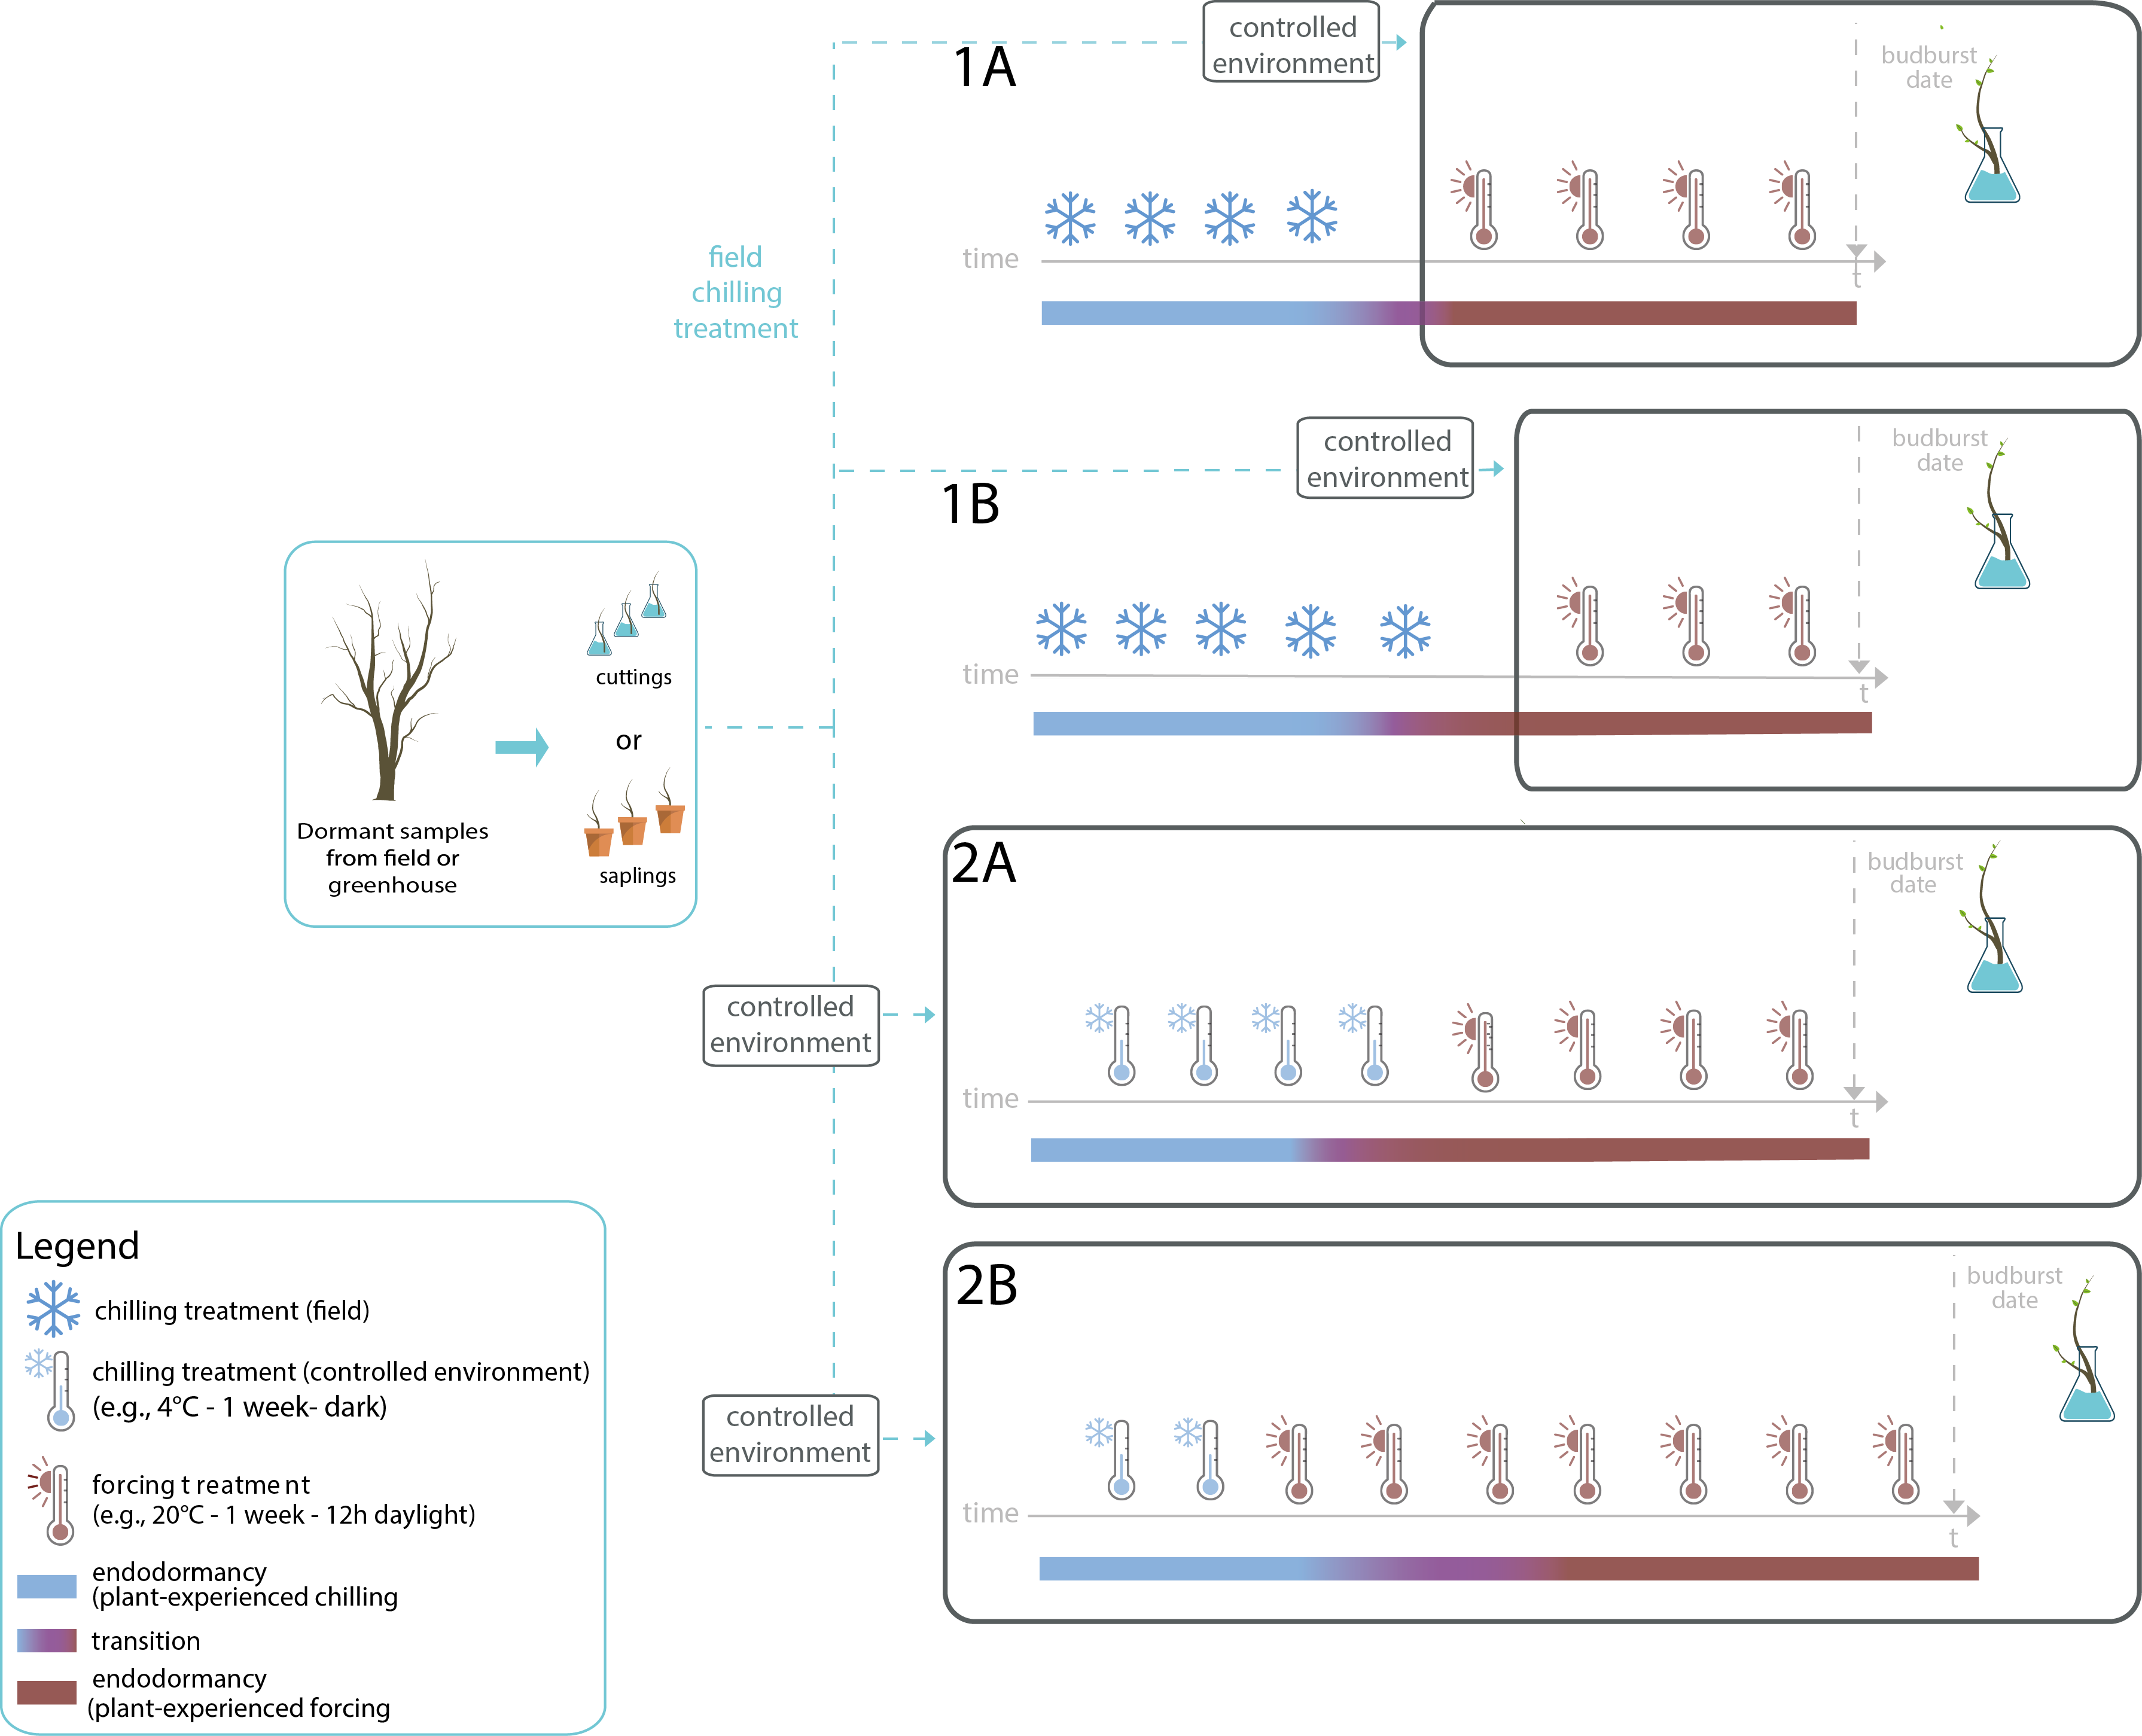
\includegraphics[width=1\textwidth]{figures/concept/Fig_bbconcept_dormant_V8.png}

\caption{\textbf{\R{ee10}Short-term experiments on woody plant phenology manipulate photoperiod and temperature to estimate chilling, forcing, and photoperiod cues.} Chilling is manipulated by using natural chilling in the field (1A-B, in which plant material is collected after different numbers of days in the fall/winter) and/or experimentally (2A-B, in which plant material is placed in controlled environment chambers set to different chilling temperatures and/or durations). Chilling treatments are designed to break plant endodormancy, after which forcing treatments are imposed by moving plant material to warmer temperatures that allow budburst to occur. Ideally, this experimental transition aligns with the physiological shift from endo- to ecodormancy (e.g., 1A, though it could also occur with experimentally applied chilling). A challenge with these experiments is that species-specific chilling requirements are rarely known, so experimental treatments may not always align with what the plant experiences (\emph{i.e.}, physiological shifts in dormancy). Thus, in some cases, chilling treatments may bridge across what plants experience as both chilling and forcing (1B and 2A, where plants transition into ecodormancy before ``forcing'' treatments are applied), or chilling treatments may end before endodormancy is fully broken (2B). In the \R{ee11}experiments synthesized here, photoperiod (not shown) is most often manipulated in forcing treatments. Across 72 studies examined, we found treatments varied uniquely for each study, but some were more common than others, see Fig. \ref{fig:treatheatmaps}: chilling treatments averaged 71.4 days (range: 1-182 days) at an average temperature of 4.4 \degree C (range: 0-16 \degree C), forcing treatments averaged 15.7 \degree C (range: 5 to 32 \degree C).}
\label{fig:concept} 
\end{figure}

\begin{figure}[h!]
\centering
\noindent 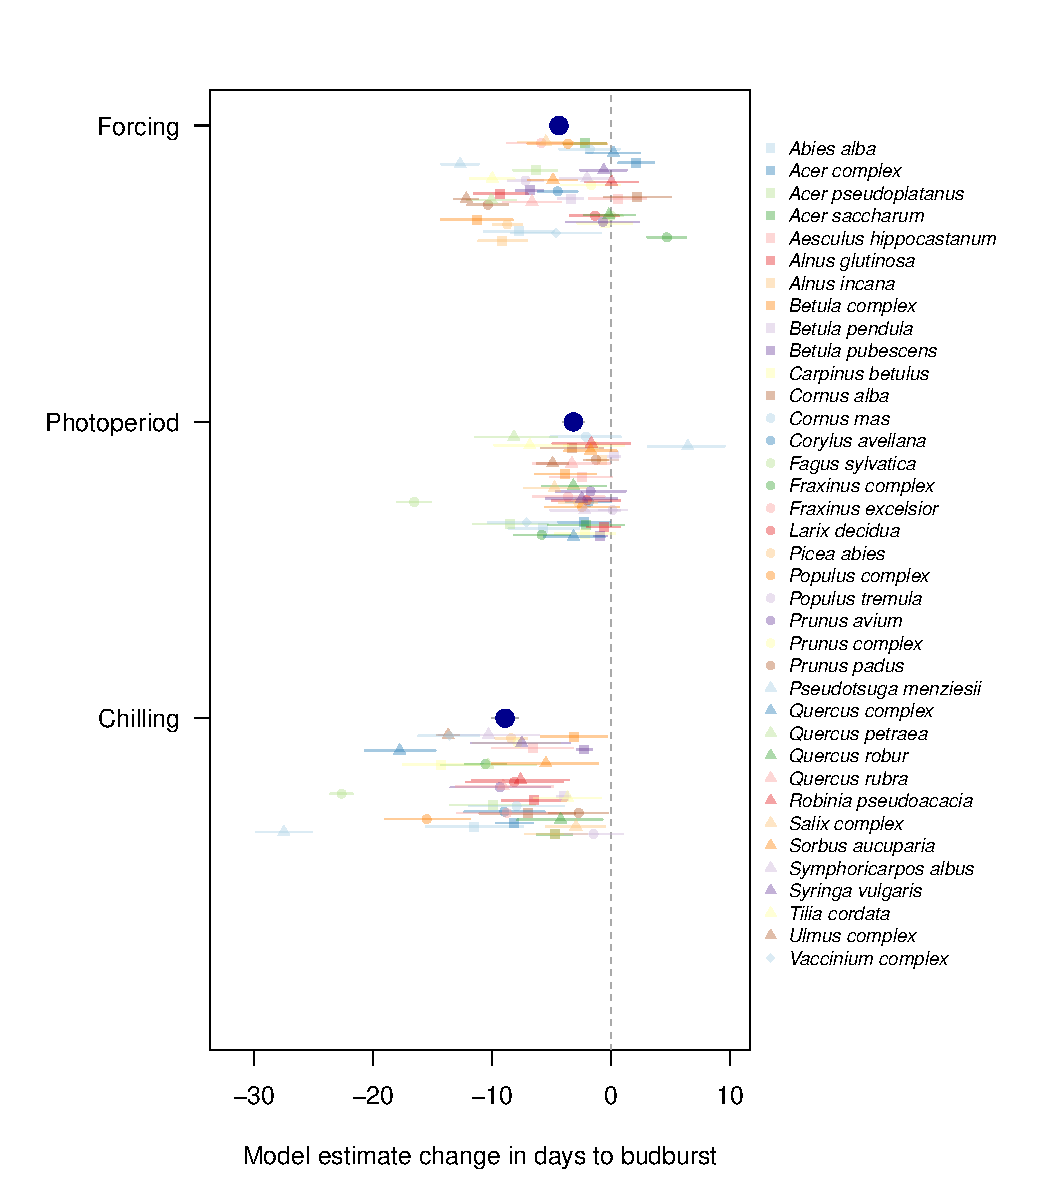
\includegraphics[width=0.75\textwidth]{..//..//analyses/bb_analysis/figures/muplotspcompexprampfputah_z.pdf}
\caption{\textbf{Estimated effects of chilling, forcing, and photoperiod on budburst timing across 65 species (modeled as 36 separate taxa, see \emph{Models} in the Supplemental Materials) in 39 controlled environment experiments\R{ee12}.} Using standardized units, which allow comparisons across cues, we show that most species (smaller symbols) are responsive to most cues, with chilling being the strongest cue when considering overall estimates across species (larger, dark blue circles). Overall estimates shown here were generally similar to other model formulations, including using data from 203 species (and 72 studies), and using different methods for calculating chilling (Figs. \ref{fig:lat}, \ref{fig:weinberger}; Tables \ref{tab:modsz}-\ref{tab:stage}). Lines represent 50\% uncertainty intervals (other intervals provided in Tables \ref{tab:modsz}-\ref{tab:stage})}. % EMW: This could be a place to sneak in another node to the study vs. species issue R1 raised. 
\label{fig:mu}
\end{figure}

\newpage
%get min bb doy and associated chilling/forcing T


\begin{figure}[h!]
\centering
\noindent 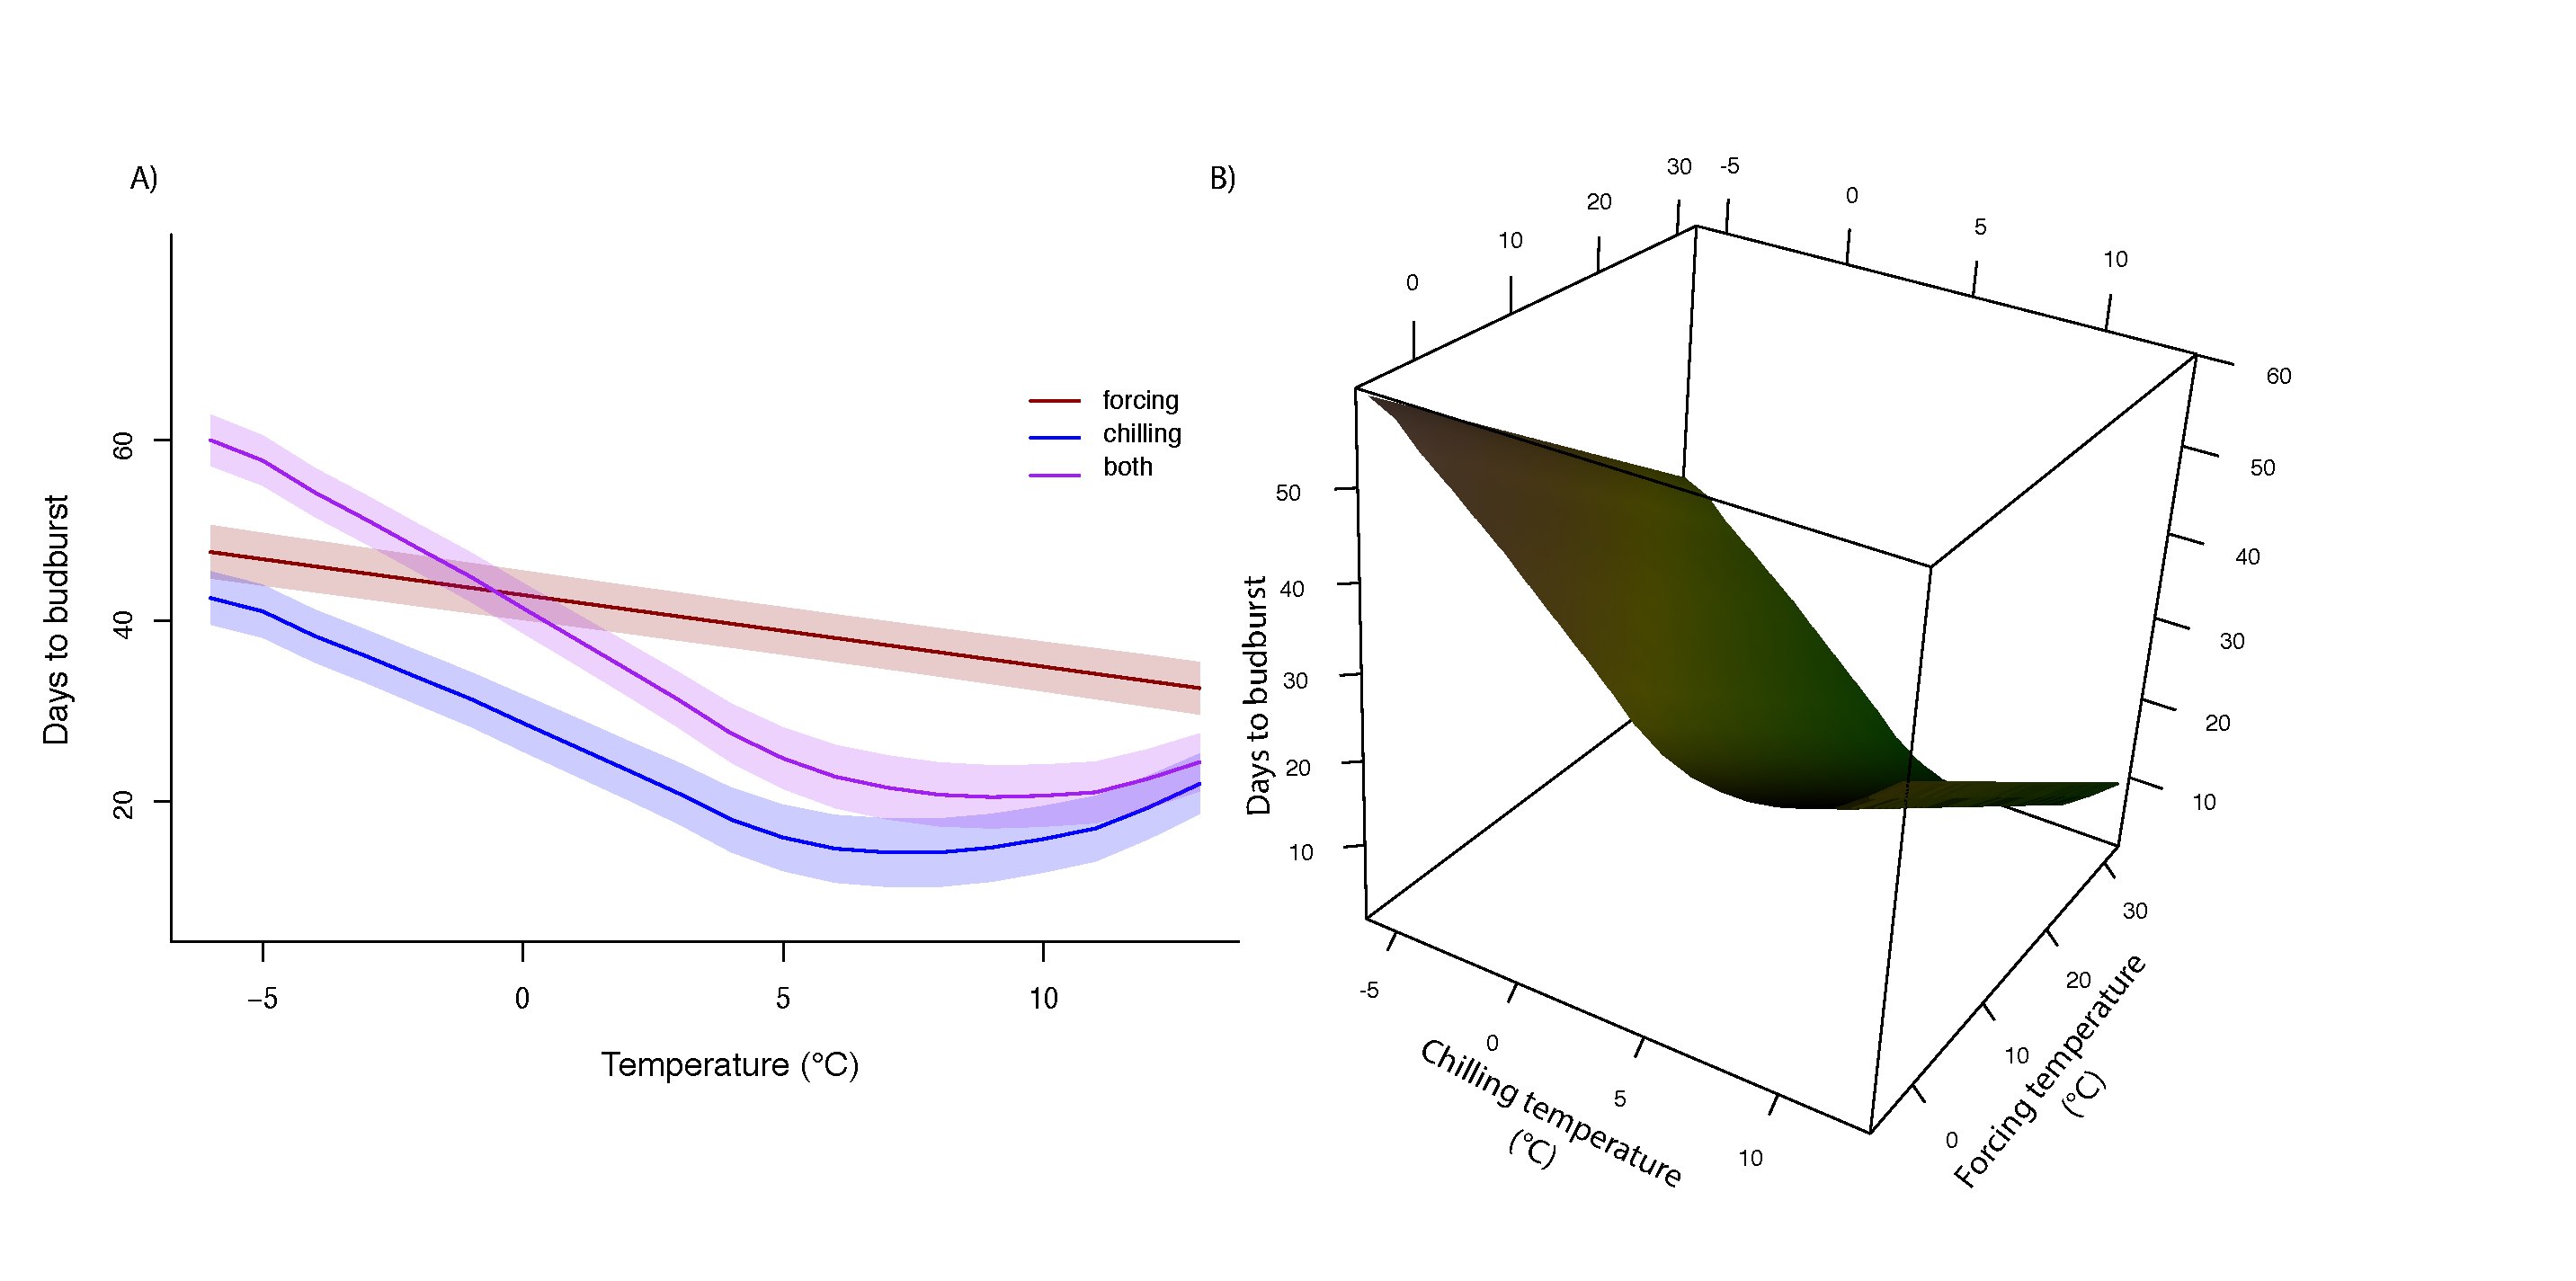
\includegraphics[width=1\textwidth]{..//..//analyses/bb_analysis/figures/bbmod_2d3dplot_utah_withPEP.pdf}
\caption{\textbf{Estimates of budburst across a range of forcing temperatures and estimated chilling} (converted to a representative mean temperature, see \emph{Estimating chilling} in Methods and Supplemental Materials) based on overall estimates of chilling and forcing effects from a meta-analysis of short-term experiments using controlled temperature and/or photoperiod conditions\R{ee13} (Fig. \ref{fig:mu}). Note that days to budburst is relative to experimental methods and thus not comparable to day of year in the field, shading (in A) represents 50\% uncertainty intervals. Panel A shows the effect of chilling temperature on budburst, with forcing kept at the mean level across all experiments (16\degree C); the effect of forcing temperature with chilling kept at the mean level across all experiments (1324 chilling units), and the effect of varying both chilling and forcing temperatures simultaneously. Panel B shows all possible combinations of chilling and forcing across the experimental conditions.
Maximum advances in budburst occur at intermediate chilling temperatures (\emph{e.g.}, here at mean winter temperatures of 6-7\degree C) and the highest forcing (here at 32\degree C). We set photoperiod to eight hours, which is the most common photoperiod treatment in our meta-analysis.} % wordcount=XXX 
\label{fig:3dfieldchillutah}
\end{figure}


\begin{figure}[h!]
\centering
\noindent 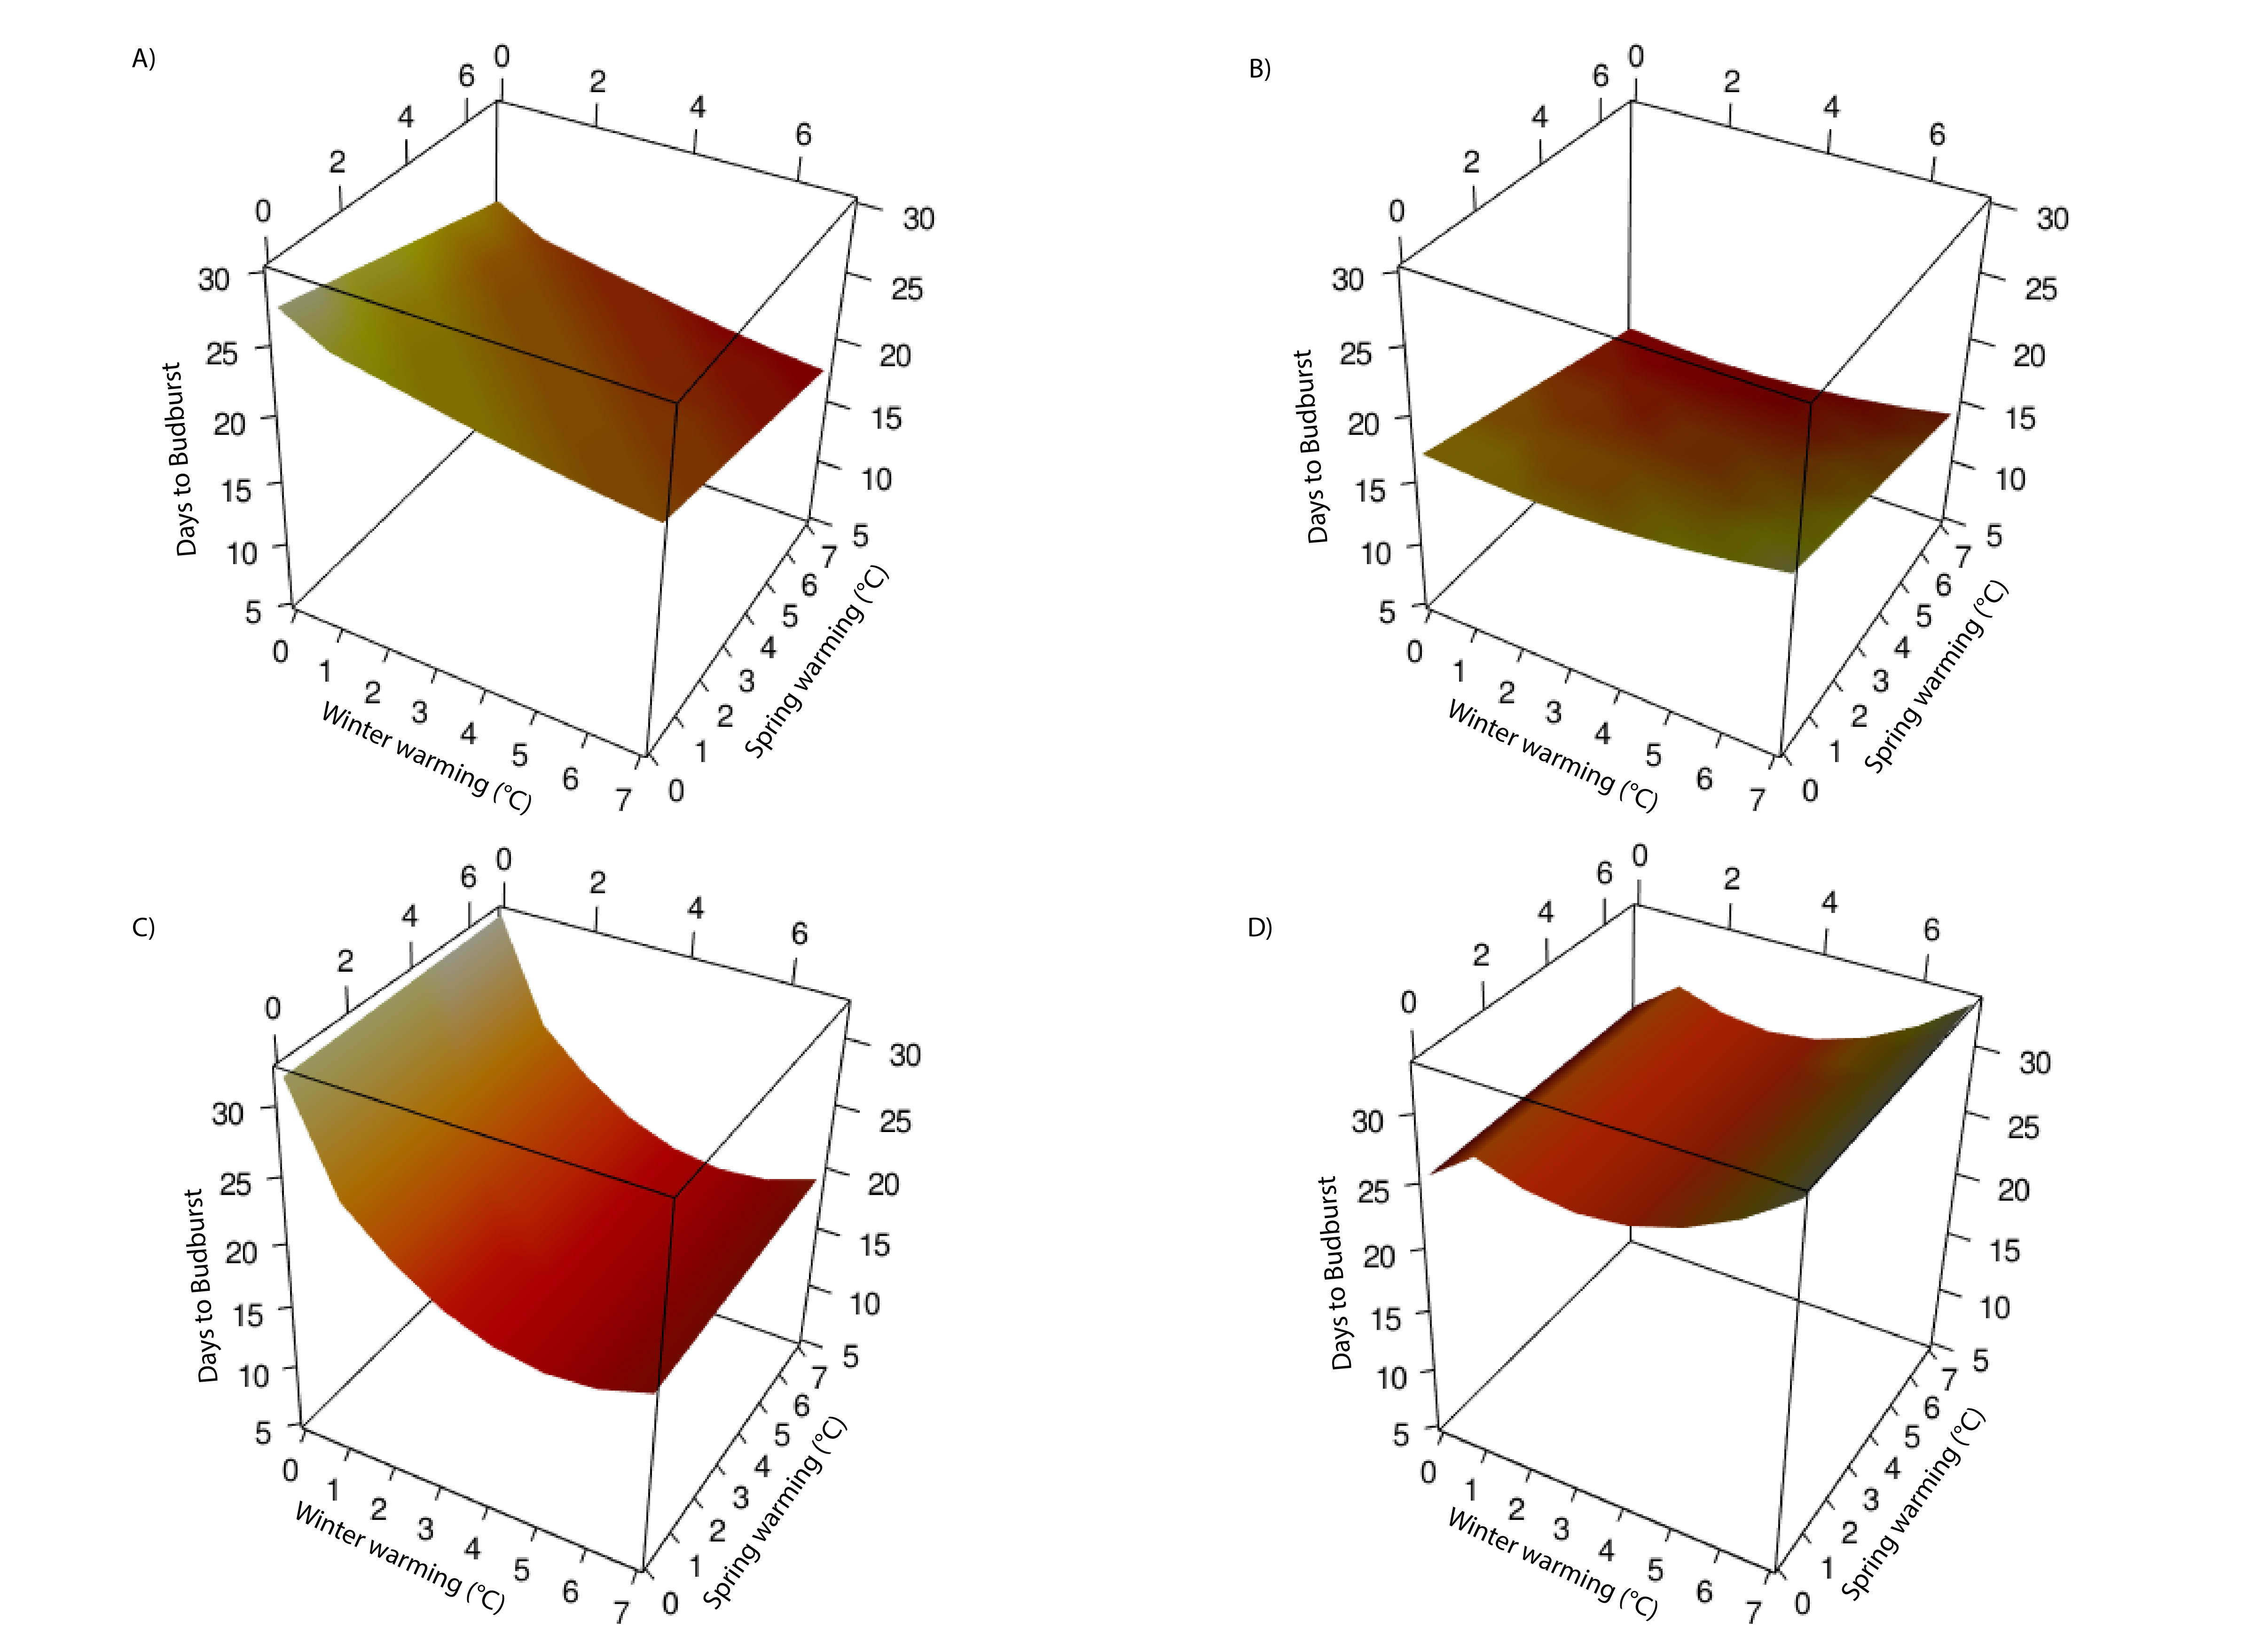
\includegraphics[width=0.75\textwidth]{..//..//analyses/bb_analysis/figures/forecasting/tempforecastbothspp_1_7_degwarm3D_utah.png}
\caption{\textbf{Implications of warming on budburst timing varies across species and sites}, depending strongly on pre-warming climate conditions related to chilling for each site. Here we show species-level estimates from our model based on a meta-analysis of experiments\R{ee14} (Fig. \ref{fig:mu}) for two common species \emph{Betula pendula} (A, B) and \emph{Fagus sylvatica} (C, D), based on climate data from two sites in Central Europe (these two sites chosen to highlight the diversity of possible budburst responses to warming, see Fig. \ref{fig:foremap} for general trends across many sites in the same region). In some sites, warming increases total chilling estimates (A, C) leading to greater advances in budburst (compared to forcing alone), whereas warming decreases total chilling estimates in other sites (B, D), leading to smaller advances and, eventually, delays with substantial warming. See Fig. \ref{fig:betfag2d} in the Supplemental Materials for a simplified two-dimensional version.}
\label{fig:betfag3d}
\end{figure}

%%%%%%%%%%%%%%%%%%%%%%%%%%%%%%%%%%%%%%%%
\end{document}
%%%%%%%%%%%%%%%%%%%%%%%%%%%%%%%%%%%%%%%%
